\documentclass[12pt, letterpaper, titlepage]{article}
\usepackage[utf8]{inputenc}
\usepackage{graphicx}
\usepackage{caption}
\usepackage{amsmath}
\usepackage{listings}
\usepackage[detect-all,per-mode=symbol]{siunitx}
\graphicspath{{./}}
%\usepackage[super,comma,sort&compress]{natbib}
\lstset{language=Python, basicstyle={\small\ttfamily}}
\usepackage{fancyhdr}
\pagestyle{fancy}
\lhead{Team 162}

\begin{document}

\begin{titlepage}
\begin{center}
\vspace*{2.7in}
{\LARGE Team 162} \\
\vspace{0.1in}
{\Large Problem B} \\
\vspace{0.55in}
{\large Composting Efficiency in a Collapsing Self-Heating Pile} \\
\vspace{0.3in}
{\large November 11, 2018}\\
\vspace{0.55in}
{A compost pile is -----}
\end{center}
\end{titlepage}

%(1) a restatement and clarification of the problem as interpreted by the team, (2) an explanation of all assumptions and approximations made, (3) justification for all work performed, as well as (4) a discussion of the strengths and weaknesses of the approach taken. 

\section{Introduction}
Composting uses biological processes to break down organic waste and turn it into a soil fertilizer. A variety of factors affect the efficiency of the composting process, including temperature, aeration, humidity, waste components, etc. Since the pile size affect its internal pressure, we expect more air voids in smaller piles, which promotes aeration. On the other hand, we expect bigger and taller piles to have a large volume to surface area ratio, thus maintaining the heat which is crucial for bacteria activity.
We interpret the given problem as follows. Given waste material with fixed mass and given the same amount of time for it to decompose under known ambient temperatures, we want to minimize the final mass of the pile as we vary the height of the pile $H$. In addition, we want to determine how the optimum piling height varies with changing dry mass content $d_{s} =$ (mass of solids)/(total mass).

\section{Assumptions}
We proceed to make the following assumptions:
\begin{enumerate}
    \item The pile is piled into a rectangle. We only want to study the effect of scaling to the efficiency, so the geometry of the pile is irrelevant.
    \item The pile under study only has two dimensions. Only the height and one of the horizontal dimensions are kept. Therefore the pile is exposed on three sides in air and one side to the ground. This two dimensional pile can be thought of as a vertical slice through the center of the actual three dimensional pile.
    \item The ratio of mass of dry solids to total mass is constant throughout the extent of the composting process.
    \item Heat transfer occurs only by conduction. The air voids within the compost material is too small for a convective circulation to develop.
\end{enumerate}
\newpage
\section{Parameter Values}
 \captionof{table}{Composition and the mechanical properties of the compost pile.} \label{table-1}
\begin{center}
    \begin{tabular}{ | l | p{3.5cm}| l |l|l|l|} 
    \hline
    Symbol & Name & Value & Unit & Source\\ \hline
    $d_s$ & dry mass density &  $0.3-0.6$  & kg/kg & est.\\ \hline
    $\gamma_s$ & density of solid compost  & 1150 & \si{\kg\per\m\cubed} & \cite{burning}  \\ \hline
    $\gamma_g$ & density of air & 1.17 or 0 & \si{\kg\per\m\cubed} & \cite{burning} with est. \\ \hline
    $\gamma_l$ & density of liquid & 1 & \si{\kg\per\m\cubed} & est.  \\ \hline
    $\rho_{min}$ & bulk mass density on top & 100 & \si{\kg\per\m\cubed} & est. \\ \hline
    $E$ & resistance against deformation  & $73$ & $ \si{\J\per\kg}^4$ & \cite{pile} \\ \hline
    %------
    \end{tabular}
\end{center}
\newpage
\captionof{table}{Constants microbes-compost system used in the evolution of the pile.} \label{table-2}
\begin{center}
    \begin{tabular}{ | l | p{3.5cm}| l |l|l|l|} 
    \hline \cite{pile}
    Symbol & Name & Value & Unit & Source\\ \hline
    $X_{0}$ & bacteria population at t=0 & 1-2 & \si{\mol\per\meter\cubed} &\cite{lin}\\ \hline
    $K_{O_{2}}$ & half-saturation constant for oxygen &  $\num{1e2}$  & mg/L & \cite{lin}\\ \hline
    $K_{\rho}$ & half-saturation constant for solid mass &  $\num{0.056}$  & \si{\kg\per\meter\cubed} & \cite{lin}\\ \hline
    
    $k_c$ & effective thermal conductivity of compost  & 0.3 & \si{\W\per\m\per\K} & \cite{burning}  \\ \hline
    $k_{air}$ & effective thermal conductivity of compost  & 0.026 & \si{\W\per\m\per\K}& \cite{burning} \\ \hline
    $C_c$ & heat capacity for compost material  & 3320 & \si{\J\per\kg\per\K}& \cite{burning} \\ \hline
    $C_{air}$ & heat capacity for air  & 1005 & \si{\J\per\kg\per\K} & \cite{burning} \\ \hline
    
    $D_{0,air}$ &  diffusion coefficient for oxygen& \num{1.98e-5} & \si{\m\squared\per\s} & \cite{Wikipedia} \\ \hline
    $A_{O_{2}}$ & ambient oxygen concentration & \num{0.272} & \si{\kg\per\meter\cubed} & \cite{burning}\\ \hline
    $W_{O_{2}}$ & dissolved oxygen concentration & \num{9.3} & \si{\mg\per\L} & \cite{ecology}\\ \hline
    $\mu_{m}$ & microbes maximum growth rate & \num{1e-4} & \si{\per\s} & \cite{lin}\\ \hline
    $b$ & microbes death rate & \num{7.6e-5} & \si{\per\s} & \cite{lin}\\ \hline
    $Y_O$ & microbes yield on oxygen & 1.12 & mol/mol & \cite{lin} \\ \hline
    %$r_{c}$ & combustion rate & 0.6 & - & estimation \\ \hline
    \end{tabular}
\end{center}

\section{Collapsing Pile}
Due to the compression of gravity, the pile of kitchen vegetable has different bulk density $\rho=M/(AH)$ as a function of the total height of the pile. To quantitatively take into account this factor, we define the following identities that describe the composition of the compost pile.
\begin{align}
    \theta_s+\theta_l+\theta_g &= 1 \\
    \gamma_s\theta_s+\gamma_l\theta_l+\gamma_g\theta_g &= \rho \label{brho-relationship}\\
    d_{\mathrm{s}} = \frac{\gamma_s\theta_s}{\rho} &= \mathrm{Constant}
\end{align}
Here we assume that the dry mass density $d_s$, the mass density of solid phase in the compost pile, to be constant, but $\theta_l$ and $\theta_g$, the volume fraction of the corresponding phase, are allowed to change. \\
The water content of the pile $w$ (\%) is given by Eq.\ref{brho-relationship} and by taking $\gamma_g\approx0$ because it's much smaller than $\gamma_s$ and $\gamma_l$. 
    \begin{equation}
        w = \frac{\theta_l\gamma_l}{\rho} = 1-d_s
    \end{equation}
The diffusion coefficient of oxygen depends on $\theta_g$, can also be derived from the algebraic relationship above. 
     \begin{equation}
        \theta_g = 1-\Big(\frac{d_s}{\gamma_s}+\frac{1-d_s}{\gamma_l}\Big)\rho \label{thetaG}
    \end{equation}
    With compression coefficient $E$ identified by \cite{pile}, we can calculate the relationship between $\rho(z)$ and total height $H$ given the uncompressed bulk density of the compost $\rho_{min}=\rho(H)$ by using force balance equation in $z$.
    \begin{equation*}
    \frac{\partial}{\partial z}\rho(z)+\frac{g}{Ed_s}\rho(z)=0
    \end{equation*}
    Integrate with respect to $z$, we can get pile mass $M$ as a function of total height $H$ and the inverse function:
    $$M = A\rho_{\mathrm{min}}\frac{\exp(\frac{gH}{Ed_{\mathrm{s}}})-1}{g/Ed_{\mathrm{s}}}$$
    \begin{equation}
        H = \frac{d_sE}{g}\mathrm{ln}\Big(1+\frac{gM}{(A\rho_{min}Eds)}\Big) \label{HofM}
    \end{equation}
    And we make the assumption that the pile density varies little in the pile and use $M/(AH)$ as the bulk density of the pile in the following calculations.
\section{Compost Dynamics}
%Given an initial height $H$ and the base area $A$ of the compost pile, we can find from the collapsing pile a corresponding total mass 
%$$M = A\rho_{\mathrm{min}}\frac{\exp(\frac{gH}{Ed_{\mathrm{s}}})-1}{g/Ed_{\mathrm{s}}}$$
%The void fraction of the bulk is calculated by %$$\theta_{\mathrm{g}} = 1-\left(\frac{d_{\mathrm{s}}}{\gamma_{\mathrm{s}}}+\frac{1}{\gamma_{\mathrm{l}}}-\frac{d_{\mathrm{s}}}{\gamma_{\mathrm{l}}}\right)\frac{M}{HA}$$
We want to model the consumption of this mass by considering the spatial and temporal evolution of the biomass density $X(\vec{r}, t)$ [mol/m$^3$], the bulk oxygen concentration $O_2(\vec{r}, t)$ [kg/m$^3$], and the temperature $T(\vec{r}, t)$ [K].
The growth and death rates of microbes in the compost can be modeled by \cite{lin}
$$R_{\mathrm{G}}(X, O_2, T, M) = \mu_{\mathrm{m}}\frac{d_{\mathrm{s}}M/(AH)}{d_{\mathrm{s}}M/(AH)+K_{\rho}}\cdot\frac{O_2}{O_2+K_{O_2}}Xf_1(T)$$
$$R_{\mathrm{D}}(X, T) = bXf_2(T)$$
where $R_{\mathrm{G}}$ and $R_{\mathrm{D}}$ [mol/m$^3$-s] are the per volume growth and death rates of bio mass, $f_1(T)$ and $f_2(T)$ are unitless factors that reflect microbe activity at different temperatures. When temperature $T$ is in Celsius \cite{lin}, 
$$f_1(T) = -3.11 \times 10^{-4}T^2+3.48\times10^{-2}T+0.0265$$
$$f_2(T) = 2.142\times 10^{-4}T^2-2.356\times10^{-2}T+1.348$$
The local rate of change of biomass density in terms of the state variables is \cite{lin}
    \begin{align}
        \frac{\partial X}{\partial t}&=R_{\mathrm{G}}(X, O_2, T, M)-R_{\mathrm{D}}(X, T) \label{dXdt}
    \end{align}
The local rate of change of oxygen can be modeled as having a term proportional to $R_G$ \cite{lin} and a diffusive term. A similar proportional result can be written down for the temperature, with an addition of the diffusive term,
    \begin{align}
        \frac{\partial O_2}{\partial t} &= -c_1R_{\mathrm{G}}(X, O_2, T, M)+D_{0,\mathrm{air}}\theta_{\mathrm{g}}\nabla^2O_2 \\
        \frac{\partial T}{\partial t} &= c_2R_{\mathrm{G}}(X, O_2, T, M)+\alpha\nabla^2T
    \end{align}
where $O_2$ [kg/m$^3$] is the local concentration of oxygen, the consumption coefficient of oxygen $c_1 = m_{\mathrm{O_2}}/{Y_O}$ is the molar mass of the oxygen over the yield rate of biomass per mol of consumption of $O_2$, the multiplication of $D_{0, air}$ with $\theta_{g}$ \cite{D0air} corrects the diffusivity of oxygen in the bulk, and $c_2$ and $\alpha$ are the heat production coefficient and the heat diffusion coefficient, respectively. They are calculated as follows. The effective volumetric heat capacity of the bulk is \cite{burning} $$\rho C_{\mathrm{eff}} = \theta_{\mathrm{g}}\rho_{\mathrm{air}}C_{\mathrm{air}}+(1-\theta_{\mathrm{g}})\gamma_{\mathrm{s}}C_{\mathrm{c}}$$
where $\theta_{\mathrm{g}}$ is taken from Eq. \ref{thetaG},
$$\theta_g = 1-\Big(\frac{d_s}{\gamma_s}+\frac{1-d_s}{\gamma_l}\Big)\frac{M}{HA}$$
then the heat production coefficient is $c_2 = c_1Q/(\rho C_{\mathrm{eff}})$, given by the consumption of oxygen times the heat produced per kg of oxygen used (taken to be 14000 kJ/kg, comparable to the equivalent combustion heat of glucose \cite{heat}) for metabolism over the effective heat capacity. The coefficient of diffusion of heat is calculated by \cite{burning}
$$\alpha = \frac{\theta_{\mathrm{g}}k_{\mathrm{air}} + (1-\theta_{\mathrm{g}})k_{\mathrm{c}}}{\rho C_{\mathrm{eff}}}$$
Finally the rate of change of total mass $M$ is modeled to be proportional to the total growth of biomass in the compost
    \begin{align}
        \frac{\mathrm{d} M}{\mathrm{d} t} &= -c_3\int dV R_{\mathrm{G}}(X, O_2, T, M) \label{dMdt}
    \end{align}
where the mass consumption coefficient $c_3 = m_{\mathrm{glucose}}/(6Y_O)$ is the molar mass of glucose over six times the microbes yield rate of oxygen. The number six comes from the ratio of glucose and oxygen consumption in the reaction $\mathrm{C_6H_{12}O_6 + 6O_2 = 6CO_2 + 6H_2O}$.
Eq.\ref{dXdt} to Eq.\ref{dMdt} form a system of first order differential equations which we can solve numerically.
 

\section{Simulation}
We use a 2D grid of cell size $dV=0.05$\si{\m\cubed} and time step $dt = 30$s to illustrate the behavior of the model. This model can be considered as a thin slab from an arbitrarily long pile with width $Lx$ and height $H$.\\
The finite difference laplacian is used and Euler's method is used to evolve the system in time. The modified mass after the time evolution of the system is fed back into the system as an initial mass. A new height is calculated from the last equation from Eq.\ref{HofM}. The parameters of simulation are recalculated before another time step is made. \\ [5px]
\begin{figure} \label{ long-term-fig} 
  \begin{minipage}[b]{0.5\linewidth}\centering
    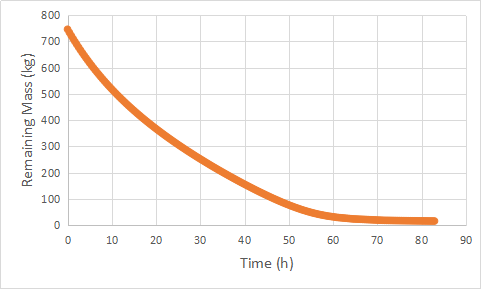
\includegraphics[width=1\linewidth]{long-m} 
  \end{minipage} 
  \begin{minipage}[b]{0.5\linewidth}\centering
    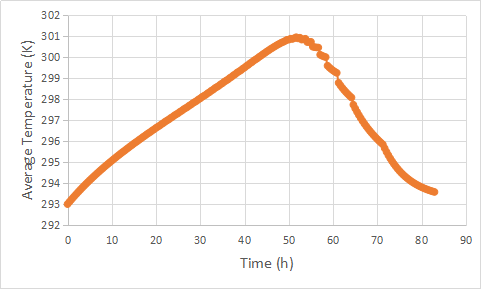
\includegraphics[width=1\linewidth]{long-k} 
  \end{minipage} 
  \begin{minipage}[b]{0.5\linewidth}\centering
    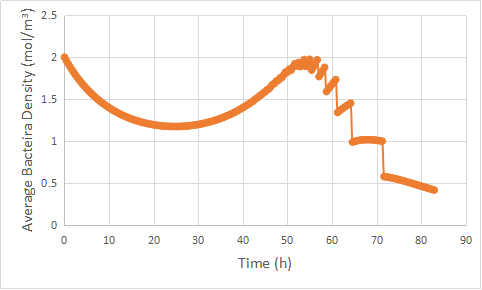
\includegraphics[width=1\linewidth]{long-o} 
  \end{minipage}
  \hfill
  \begin{minipage}[b]{0.5\linewidth}\centering
    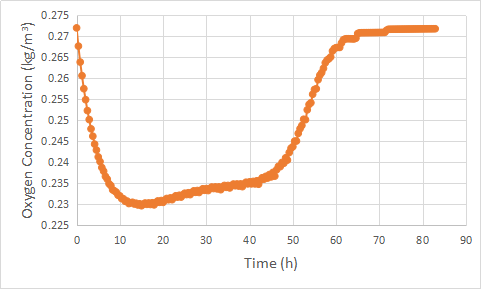
\includegraphics[width=1\linewidth]{long-x} 
  \end{minipage} 
  \caption{ Test of long-term behavior of the model under constant ambient temperature. a) 2\% of initial mass remains after 82 hours. b) Temperature increases first due to the metabolism of the microbes and decline as the size of the pile decreases. Ambient temperature is set to be $20^{\circ}$C. c) Bacteria density in the pile. d) Oxygen concentration in the pile. Fast oxygen consumption agrees with heat production in the first phase. The discontinuity results from the finte cell size when the pile is compressed down as the mass decreases.} 
\end{figure}
\section{Results}
\begin{minipage}[h]{\linewidth}
    	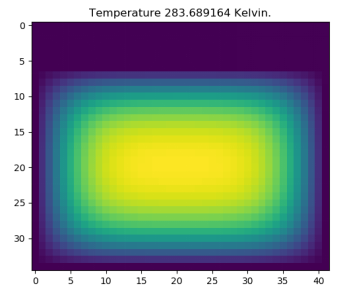
\includegraphics[scale=1]{compressed-t}
        \captionof{figure}{The temperature distribution of the compressed pile after 80 hours. Lighter colors indicate higher temperatures. The average temperature is 283.7K.}\label{tm-ply}
   	\end{minipage}
    \begin{minipage}[h]{\linewidth}
    	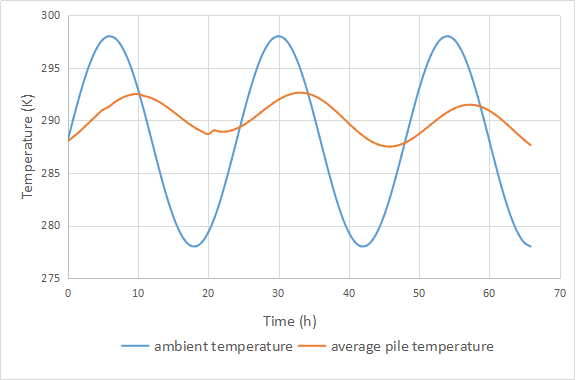
\includegraphics[scale=.8]{temp-curve}
        \captionof{figure}{Pile temperature and ambient temperature changes over time in a pile with $H=0.65$m and water content $w=0.5$. The temperature of the pile varies between $5^{\circ}$C and $20^{\circ}$C over the 24 hour period and the pile temperature changes accordingly. The gradual decrease in pile temperature is the result of decreasing height and therefore enhanced heat loss.\\}\label{tm-ply}
   	\end{minipage}
   	We consider the water content of the compost pile to vary between 40\% and 70\% and search for the optimal height of the pile to minimize the percentage of compost remain after 67 hours.
   	\begin{minipage}[h]{\linewidth}
    	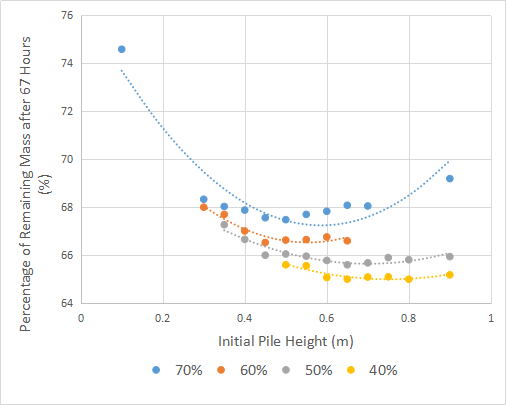
\includegraphics[scale=1]{opt-curve}
        \captionof{figure}{Different compost efficiency with varying pile shape and input material. The data points represent the result of each simulation and the dotted lines are parabola fitting curves, showing a local minimum at around 0.57m for $w=70\%$, 0.55m for $w=60\%$, 0.65m for $w=70\%$, and 0.7m for $w=70\%$.\\}\label{tm-ply}
   	\end{minipage}

\section{Discussion}
    In this complicated model, there are many ways to evaluate the efficiency. Since we are mostly concerned with kitchen vegetable waste and the feasibility in composting such waste at home. Based on the result above, we find that for material with high water content, the optimized height is higher, at around 0.7m. \\
    The complex mixture of the compost poses a challenge to simulations and theoretical development. Future models may consider larger industrial-size models and maximize total mass reduction. The evolution of bacteria colonies can be Incorporated in the model to account for varying levels of activity in the stages of composting.
    
    
\begin{thebibliography}{1}

\bibitem{lin} Y. P. Lin, G. H. Huang, H.W.Lu, L.He, ``Modeling of substrate degradation and oxygen consumption in waste composting processes." {\em Waste Management}, Vol. 28, Is. 8, pp. 1375-1385. 2008.

\bibitem{heat}  The Japan Reader, ``Modelling composting as a microbial ecosystem: a simulation approach." {\em Ecological Modelling}, Vol. 91, Is. 1–3, pp. 25-37. 1996.

\bibitem{burning} H. S. Sidhu, M. I. Nelson, X. D. Chen.``A simple spatial model for self-heating compost piles." {\em ANZIAM J.} Vol. 48, pp. C135--C150. 2007.

\bibitem{pile} J.T. Van Ginkel, P.A.C. Raats, I.A. Van Haneghem, ``Bulk density and porosity distributions in a compost pile." {\em Netherlands Journal of Agricultural Science}, Vol. 47, pp. 105-121. 1999.
\bibitem{D0air} J. Neira, M. Ortiz, L. Morales, E. Acevedo, ``Oxygen diffusion in soils: Understanding the factors and processes needed for modeling." {\em Chilean Journal of Agricultural Research}, Vol.75, Supl.1. 2015.
\bibitem{ecology} Fundamentals of Environmental Measurements, "Dissolved Oxygen", https://www.fondriest.com/environmental-measurements/parameters/water-quality/dissolved-oxygen/, Accessed Nov. 11, 2018.
\bibitem{Wikipedia} Wikipedia, "Mass Diffusivity", https://en.wikipedia.org/wiki/Mass\_diffu

sivity, Accessed Nov. 11, 2018.
\end{thebibliography}
\end{document}